\section{Experiments}
\label{sec:exp}

\subsection{Setup}
\textbf{Data.} We use LFPW~\cite{belhumeur2011lfpw} with the 300-W 68-point
re-annotation~\cite{sagonas2013_300w,sagonas2016_300w}, obtained from the Menpo
mirror~\cite{menpo_lfpw} (\cref{tab:data}). Following the 300-W protocol, which supplies a
face box, each image is cropped around the annotated face (landmark extent + 60\%);
many LFPW photos contain several people. The \textbf{train} split is used \emph{only} to
fit the 478$\to$68 map and to calibrate the gate. Every number below is computed on the
\textbf{test} split. WFLW~\cite{wu2018lab} was our first choice for its attribute subsets,
but its Google-Drive-hosted images were unreachable from our compute environment. The code
reads any 68-point \texttt{.pts} dataset.

\begin{table}[t]
\centering\footnotesize
\begin{tabular}{@{}lccl@{}}
\toprule
Split & Images & Faces detected & Used for\\
\midrule
LFPW train & 811 & 810 & 478$\to$68 map, gate calibration\\
LFPW test & 224 & 224 & all evaluation (clean)\\
Perturbed test & 5{,}824 & 5{,}730 & robustness (26 settings $\times$ 224)\\
\bottomrule
\end{tabular}
\caption{\textbf{Data.} 68 manual landmarks per face; research-use licence (300-W).}
\label{tab:data}
\end{table}

\textbf{Reference without symmetry labels.} No public dataset has ground-truth symmetry
ratings. We therefore compute the \emph{same} measure (\cref{eq:asym}) from the expert
68-point annotations, $A_{ref}$, and evaluate how well each detector-based measure agrees
with it (Spearman $\rho$, Pearson $r$, MAE). $A_{ref}$ is not ``true'' asymmetry: it
contains annotator noise and the same 2D/pose limitations (\cref{sec:discussion}). It is
the best available reference for \emph{the measurement} we want to automate.

\textbf{Perturbations} (deterministic, applied to all 224 test faces): brightness
$\times\{0.25,0.4,0.6,1.5,2,2.5\}$; Gaussian blur $\sigma\!=\!s\cdot\mathrm{IOD}/100$,
$s\!\in\!\{1,2,4,6,8\}$; a grey box over one eye, the nose or the mouth (annotation box
+35\%); in-plane rotation $\pm\{5,10,20,30\}^\circ$ on an enlarged canvas; and downscaling
$\times\{0.5,0.3,0.2,0.12\}$. The face is unchanged, so $A_{ref}$ is unchanged too.

\textbf{Metrics.} \emph{Drift}: median $|$score(perturbed)$-$score(clean)$|$ divided by the
clean between-subject SD of that variant. This is scale-free, so M0 (face-width units) and
M1/M3 (IOD units) can be compared. \emph{Reported}: fraction of images not rejected.
\emph{Silent failure}: fraction of images whose score is \emph{reported} but has
$|A-A_{ref}|>1\%$ IOD (about twice the clean MAE, fixed a priori). This is the failure a
gate must prevent. For M0, MAE and silent failure are undefined because its units differ
from those of $A_{ref}$.
\textbf{Implementation:} Python 3.13, MediaPipe 0.10.32, OpenCV 5.0, NumPy/SciPy, Streamlit
1.66; CPU only. All tables and figures are generated by scripts from the saved CSVs.

\begin{figure*}[t]
\centering
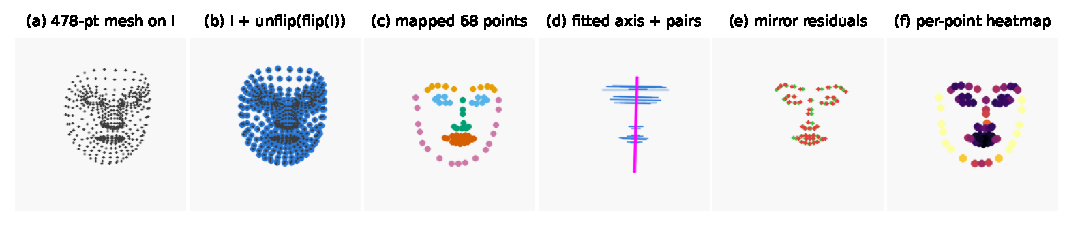
\includegraphics[width=\textwidth]{figures/pipeline_examples.pdf}
\caption{\textbf{Intermediate outputs for one test face}, drawn as geometry only.
(a) mesh on $I$; (b) mesh on $I$ (black) and unflipped mesh from $\mathrm{flip}(I)$ (blue),
almost coincident here ($\delta$ small); (c) mapped 68 points coloured by region;
(d) bilateral pairs and the fitted axis (magenta); (e) each point (green) and the
reflection of its partner (red); (f) per-point $a_i$ (bright = larger).}
\label{fig:pipeline}
\end{figure*}

\subsection{E1--E3: agreement with the annotation-based reference}
\Cref{tab:agree} and \cref{fig:agree} answer the first question: does the system measure
what we intend? The re-implemented baseline reaches $\rho$=\rhoMzero{}, or \rhoMzeroNoAlign{}
without its alignment step. Replacing only its KD-tree matching with the fixed canonical
pairs, keeping the same detections, mesh and midline, raises $\rho$ to \rhoMzeroFixed{}.
\emph{Correspondence is the dominant error source in the baseline.} The 68-point measure
with the fitted axis reaches \rhoMone{} (MAE \maeMone\% IOD), and mirror averaging reaches
\rhoMthree{}.

\begin{table}[t]
\centering\footnotesize
\setlength{\tabcolsep}{3pt}
\resizebox{\linewidth}{!}{\begin{tabular}{@{}lccc@{}}
\toprule
Measure ($n$=224) & $\rho$ & $r$ & MAE\\
\midrule
M0 baseline~\cite{nashokan_facialasymmetry} (KD-tree, vert.\ midline) & 0.823 & 0.762 & --\\
\quad M0 w/o alignment & 0.614 & 0.630 & --\\
\quad M0 + fixed pairs (no KD-tree) & 0.931 & 0.903 & --\\
M1: 68-pt pairs + fitted axis & 0.938 & 0.951 & 0.45\\
M3: M1 + mirror averaging & 0.947 & 0.957 & 0.45\\
\bottomrule
\end{tabular}
}
\caption{\textbf{Agreement with $A_{ref}$} on the clean LFPW test set (E1/E2): Spearman $\rho$, Pearson $r$, MAE in \% IOD. All rows
use identical detections.}
\label{tab:agree}
\end{table}

\begin{figure}[t]
\centering
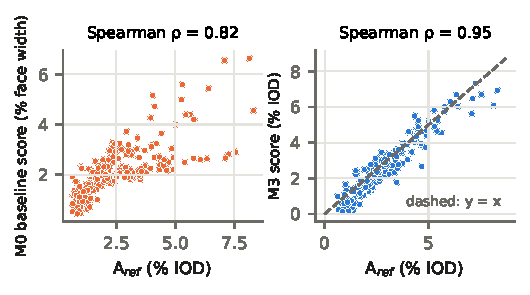
\includegraphics[width=\linewidth]{figures/agreement.pdf}
\caption{\textbf{Detector-based score vs.\ annotation-based reference} (224 test faces).
Left: baseline M0. Right: proposed M3. Points below $y\!=\!x$ show that the detector
under-estimates asymmetry.}
\label{fig:agree}
\end{figure}

\textbf{Regional analysis (E3, \cref{tab:regions}).} Regional agreement is lower than
global agreement ($\rho$ 0.84--0.98) because each region has fewer points. A systematic effect
appears: detector-based asymmetry is \emph{smaller} than annotation-based asymmetry, by
\shrinkGlobal\% globally and \shrinkMouth\% at the mouth (Wilcoxon $p<$0.01 except for the
brows, $p$=\pBrows{}). MediaPipe regresses a mesh with a strong shape prior, and this
pulls atypical (asymmetric) shapes towards the symmetric template. Part of the gap may also
be annotator noise, which inflates $A_{ref}$. Users should read detector-based regional
values as conservative.

\begin{table}[t]
\centering\footnotesize
\setlength{\tabcolsep}{3pt}
\resizebox{\linewidth}{!}{\begin{tabular}{@{}lcccccc@{}}
\toprule
 & \multicolumn{2}{c}{Spearman $\rho$} & \multicolumn{2}{c}{MAE (\% IOD)} & \multicolumn{2}{c}{mean A (\% IOD)}\\
\cmidrule(lr){2-3}\cmidrule(lr){4-5}\cmidrule(lr){6-7}
Region & M1 & M3 & M1 & M3 & ref & M3\\
\midrule
Brows & 0.840 & 0.848 & 0.76 & 0.76 & 2.85 & 2.80$^{\dagger}$\\
Eyes & 0.882 & 0.895 & 0.59 & 0.56 & 2.25 & 2.08\\
Nose & 0.912 & 0.914 & 0.87 & 0.86 & 3.90 & 3.53\\
Mouth & 0.876 & 0.889 & 0.54 & 0.56 & 1.86 & 1.36\\
Jaw & 0.974 & 0.977 & 1.61 & 1.60 & 11.73 & 10.44\\
\midrule
Global (inner 51) & -- & -- & -- & -- & 2.51 & 2.19\\
\bottomrule
\end{tabular}
}
\caption{\textbf{Regional agreement and shrinkage} (E3). Right block: mean asymmetry from
annotations vs.\ M3. $^{\dagger}$difference not significant (Wilcoxon $p\geq$0.01).}
\label{tab:regions}
\end{table}

\subsection{E8: head pose confounds 2D asymmetry}
\Cref{fig:pose} and \cref{tab:pose} show the strongest effect we observed. Even computed from
\emph{expert annotations}, 2D asymmetry follows $|$yaw$|$ almost monotonically
($\rho$=\rhoYawRef{}), from \yawLow\% IOD below 5$^\circ$ to \yawHigh\% above 20$^\circ$.
A turned head foreshortens one half of the face, and no 2D reflection can undo that. This
is a property of the \emph{quantity}, not of the detector. The detector's error relative to
$A_{ref}$ barely changes with yaw (\cref{tab:pose}), which is why a gate trained to predict
detector error would miss it. Restricting to gate-accepted images lowers the correlation to
$\rho$=\rhoYawRefAcc{}, but it does not remove it. LFPW is an in-the-wild set whose test
faces mostly have $|$yaw$|>$5$^\circ$. For a frontal capture the remaining pose effect is small,
but a ``symmetry score'' computed from an arbitrary selfie mostly measures head pose.

\begin{figure}[t]
\centering
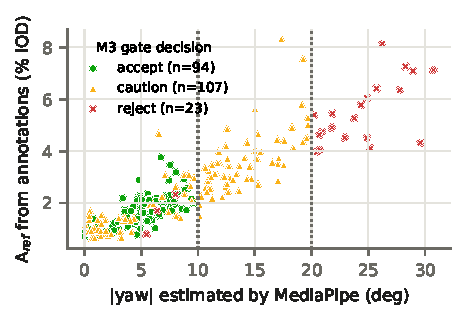
\includegraphics[width=0.95\linewidth]{figures/pose_confound.pdf}
\caption{\textbf{Asymmetry from expert annotations vs.\ estimated $|$yaw$|$} (E8), coloured
by the M3 gate decision. Dotted lines: caution (10$^\circ$) and reject (20$^\circ$) limits.}
\label{fig:pose}
\end{figure}

\begin{table}[t]
\centering\footnotesize
\resizebox{\linewidth}{!}{\begin{tabular}{@{}lccccc@{}}
\toprule
$|$yaw$|$ (deg) & n & A$_{ref}$ & M1 & $|$err$|$ M3 & NME\\
\midrule
0-5 & 77 & 1.20 & 0.80 & 0.47 & 3.03\\
5-10 & 67 & 2.14 & 1.86 & 0.40 & 5.51\\
10-20 & 60 & 3.60 & 3.41 & 0.42 & 3.32\\
$\geq$20 & 20 & 5.50 & 5.42 & 0.57 & 4.13\\
\bottomrule
\end{tabular}
}
\caption{\textbf{Pose strata} (E8, test set; values in \% IOD). Each image is
observed once, so the strata contain \emph{different} people, not the same face at several poses.}
\label{tab:pose}
\end{table}

\subsection{The mirror test detects bad landmarks without labels}
Across test images, $\delta$ correlates with the true landmark error (inner-51 NME,
$\rho$=\rhoMirrorNme{}). As a ranking signal for discarding images (\cref{fig:rc}, left),
it lowers the area under the NME risk--coverage curve from \aurcRandom{} (random) to
\aurcMirror{} (oracle: \aurcOracle{}), closing \gapClosed\% of the gap to the oracle. The
image-quality gate risk alone reaches \aurcGateTwo{}. $\delta$ predicts the
\emph{asymmetry} error much less well ($\rho$=\rhoMirrorErr{}; AURC \aurcAsymMirror{}
vs.\ \aurcAsymRandom{} random; \cref{fig:rc}, right). On clean photos, most landmark
errors are shared by the two sides of the face and cancel in $A$. The gate's value for
asymmetry shows up under degradation (\cref{sec:robust}).

\begin{figure}[t]
\centering
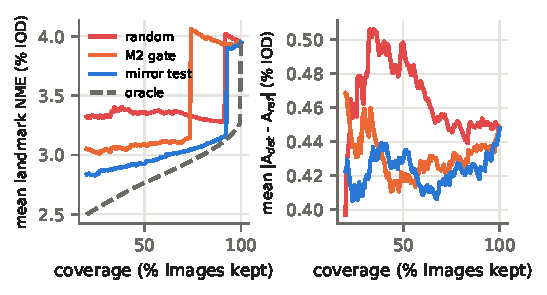
\includegraphics[width=\linewidth]{figures/risk_coverage.pdf}
\caption{\textbf{Risk--coverage on the clean test set.} Images are kept in order of
increasing risk; the y-axis is the mean error of the kept set (lower is better).
Left: landmark NME. Right: asymmetry error $|A_{det}-A_{ref}|$.}
\label{fig:rc}
\end{figure}

\subsection{E4--E7, E9: robustness and ablation}
\label{sec:robust}
\Cref{fig:robust} and \cref{tab:ablation} summarise 5{,}824 perturbed measurements.
MediaPipe is remarkably robust: it still finds a face in $\geq$\detMin\% of the images in
every setting (lowest: blur $s$=8). The danger is therefore not a missing result but a
\emph{plausible-looking wrong} one. Without a gate (M1), \silentPoolOne\% of all perturbed
measurements are silent failures, rising to \silentBlurOne\% under blur. The gate (M2/M3)
lowers this to \silentPoolTwo\%/\silentPoolThree\% (blur: \silentBlurThree\%; downscaling:
\silentDownOne\%$\to$\silentDownThree\%). The cost is coverage: \covPoolThree\% of perturbed
and \covCleanThree\% of clean images still receive a score. On clean images silent
failures fall from \silentCleanOne\% to \silentCleanThree\%.
\textbf{Mirror averaging} lowers the median drift from \driftPoolOne{} to \driftPoolThree{}
SD (\driftReduction\% less, pooled) and helps under \emph{every} perturbation type.
\textbf{In-plane rotation} (E7): a vertical-midline measure without alignment drifts by up
to \rotNoAlignMax{} SD at 30$^\circ$. The baseline's align-and-re-detect step fixes this, at
the cost of a second detection. The fitted axis achieves the same stability (M3 $\leq$
\rotMthreeMax{} SD) with no re-detection.

\begin{figure*}[t]
\centering
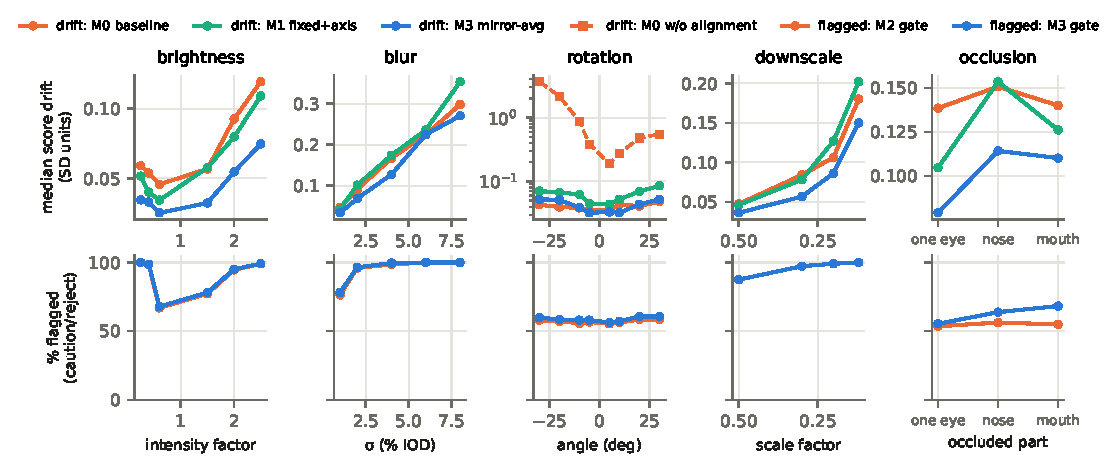
\includegraphics[width=0.92\textwidth]{figures/robustness.pdf}
\caption{\textbf{Controlled perturbations} (E4--E7; 224 test faces per point). Top:
median score drift in units of the clean between-subject SD (rotation panel in log scale;
dashed: vertical-midline baseline without alignment). Bottom: share of images the gate
flags as caution or reject.}
\label{fig:robust}
\end{figure*}

\begin{table}[t]
\centering\scriptsize
\setlength{\tabcolsep}{2.2pt}
\resizebox{\linewidth}{!}{\begin{tabular}{@{}llcccccc@{}}
\toprule
Setting & Var. & n & Reported & Accepted & $\rho$ & Silent fail. & Drift\\
 & & & (\%) & (\%) & vs ref & (\%) $\downarrow$ & (SD) $\downarrow$\\
\midrule
Clean test & M0 & 224 & 100.0 & 100.0 & 0.823 & -- & --\\
 & M1 &  & 100.0 & 100.0 & 0.938 & 5.8 & --\\
 & M2 &  & 90.2 & 43.3 & 0.921 & 4.9 & --\\
 & M3 &  & 89.7 & 42.0 & 0.932 & 4.0 & --\\
\midrule
Perturbed, pooled & M0 & 5824 & 98.4 & 98.4 & 0.814 & -- & 0.070\\
 & M1 &  & 98.4 & 98.4 & 0.921 & 8.1 & 0.076\\
 & M2 &  & 64.0 & 22.6 & 0.918 & 3.4 & =\\
 & M3 &  & 63.2 & 21.0 & 0.927 & 3.6 & 0.054\\
\midrule
\quad blur & M0 & 1120 & 94.0 & 94.0 & 0.787 & -- & 0.131\\
 & M1 &  & 94.0 & 94.0 & 0.870 & 14.4 & 0.130\\
 & M2 &  & 37.0 & 5.8 & 0.903 & 2.7 & =\\
 & M3 &  & 35.6 & 5.2 & 0.919 & 2.3 & 0.099\\
\midrule
\quad downscale & M0 & 896 & 98.7 & 98.7 & 0.821 & -- & 0.087\\
 & M1 &  & 98.7 & 98.7 & 0.909 & 9.2 & 0.097\\
 & M2 &  & 33.5 & 4.0 & 0.919 & 1.8 & =\\
 & M3 &  & 33.4 & 4.0 & 0.927 & 1.9 & 0.066\\
\midrule
\quad brightness & M0 & 1344 & 99.5 & 99.5 & 0.818 & -- & 0.065\\
 & M1 &  & 99.5 & 99.5 & 0.936 & 5.8 & 0.056\\
 & M2 &  & 62.8 & 10.6 & 0.927 & 2.8 & =\\
 & M3 &  & 62.4 & 10.2 & 0.940 & 2.7 & 0.037\\
\midrule
\quad occlusion & M0 & 672 & 98.8 & 98.8 & 0.804 & -- & 0.142\\
 & M1 &  & 98.8 & 98.8 & 0.919 & 8.8 & 0.124\\
 & M2 &  & 87.9 & 45.1 & 0.900 & 6.2 & =\\
 & M3 &  & 85.1 & 37.5 & 0.911 & 6.0 & 0.098\\
\midrule
\quad rotation & M0 & 1792 & 100.0 & 100.0 & 0.825 & -- & 0.039\\
 & M1 &  & 100.0 & 100.0 & 0.944 & 5.2 & 0.059\\
 & M2 &  & 88.1 & 43.0 & 0.924 & 4.0 & =\\
 & M3 &  & 87.7 & 41.4 & 0.928 & 4.9 & 0.040\\
\bottomrule
\end{tabular}
}
\caption{\textbf{Ablation} (E9). Reported = not rejected; Accepted = no caution.
Silent fail.: reported \emph{and} $|A-A_{ref}|>$1\% IOD. Drift: median, in clean-SD units
(``='': same score as M1).}
\label{tab:ablation}
\end{table}

\textbf{Gate behaviour on clean photos.} On the clean test set M3 accepts \pAccept\%,
cautions \pCaution\% and rejects \pReject\% of the faces. The mean NME of accepted faces
is \nmeAccept\% vs.\ \nmeCaution\% for caution. \Cref{tab:reasons} lists the triggers;
pose dominates, consistent with E8. \Cref{fig:gate} shows one face per decision.

\begin{table}[t]
\centering\footnotesize
\begin{minipage}{0.45\linewidth}\centering
\resizebox{\linewidth}{!}{\begin{tabular}{@{}lcc@{}}
\toprule
Signal & caution & reject\\
\midrule
$|$yaw$|$ & 60 & 20\\
$|$pitch$|$ & 41 & 2\\
mirror inconsistency $\delta$ & 12 & 1\\
face size (IOD) & 16 & 0\\
over-exposure & 10 & 0\\
sharpness & 7 & 0\\
several faces & 6 & 0\\
clipped pixels & 4 & 0\\
under-exposure & 3 & 0\\
\bottomrule
\end{tabular}
}
\end{minipage}\hfill
\begin{minipage}{0.53\linewidth}
\caption{\textbf{Which signal triggered the gate} on the 224 clean test faces (one image can
trigger several).}
\label{tab:reasons}
\end{minipage}
\end{table}

\begin{figure}[t]
\centering
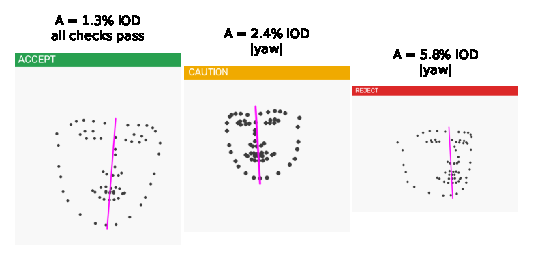
\includegraphics[width=\linewidth]{figures/gate_examples.pdf}
\caption{\textbf{Gate decisions} for three test faces (the median-$|$yaw$|$ face of each
class), drawn as landmarks + fitted axis.}
\label{fig:gate}
\end{figure}

\textbf{Region validity under occlusion: a negative result.} When the nose or the mouth
is occluded, $\delta_r$ marks that region unreliable in \occNose\% and \occMouth\% of the
faces, against \occNoseOther\% and \occMouthOther\% for the other regions. When an
\emph{eye} is occluded it does so in only \occEye\% of faces. MediaPipe fills in the
hidden eye from its shape prior, and does so consistently in both the original and the
mirror image. The mirror test detects \emph{inconsistent} landmarks, not
\emph{confidently invented} ones. Occlusion needs an appearance-based check (future work).
